\chapter{Analyse}
\label{ch:analysis}

Afin de structurer et formaliser les besoins des utilisateurs dans le but d'assurer la compréhension entre les différents partis, j'ai choisi de les représenter sous forme de diagrammes \gls{a-uml}. L'\gls{a-uml} est un standard d'industrie qui permet de représenter des informations de manière univoque. Bien que ce soit sensé être un standard, les différentes implémentations disponibles sur le marché se distinguent les unes des autres et il peut être utile de noter que j'ai utilisé le logiciel \guillemotleft{} Visual Paradigm Modeler Edition \guillemotright{} en version 15.2.

\section{Les cas d'utilisation}
\label{sec:use-cases}

\paragraph{}
Le seul besoin métier est la validation de fichiers Excel contenant des données utiles à l'accomplissement du travail de l'utilisateur. Toutefois, la mise en place d'un site web implique la gestion d'autres aspects comme la sécurité ou l'administration du site web.

\paragraph{}
On distingue trois types d'utilisateurs qui n'ont pas accès aux mêmes fonctionnalités:
\begin{itemize}
    \item Le \textbf{visiteur}: Il n'a accès à rien si ce n'est l'accès à l'authentification afin de gagner les privilèges de l'\textbf{utilisateur}.
    \item L'\textbf{utilisateur}: Il a accès aux fonctionnalités qui font le coeur de l'application. Cette dernière est conçu pour lui.
    \item L'\textbf{administrateur}: Il a tous les droits de l'utilisateur normal avec en plus la possibilité d'accéder aux outils d'administration qui permettent notamment de modifier les paramètres du serveur ainsi que les utilisateurs eux-même.
\end{itemize}

A partir d'ici, je mettrai ces trois termes en gras lorsque je ferai explicitement référence aux définitions présentes ci-dessus plutôt qu'à celles de la langue française.

\subsection{La liste des cas d'utilisation}
\label{subsec:use-cases-list}

\begin{figure}[ht]
    \centering
    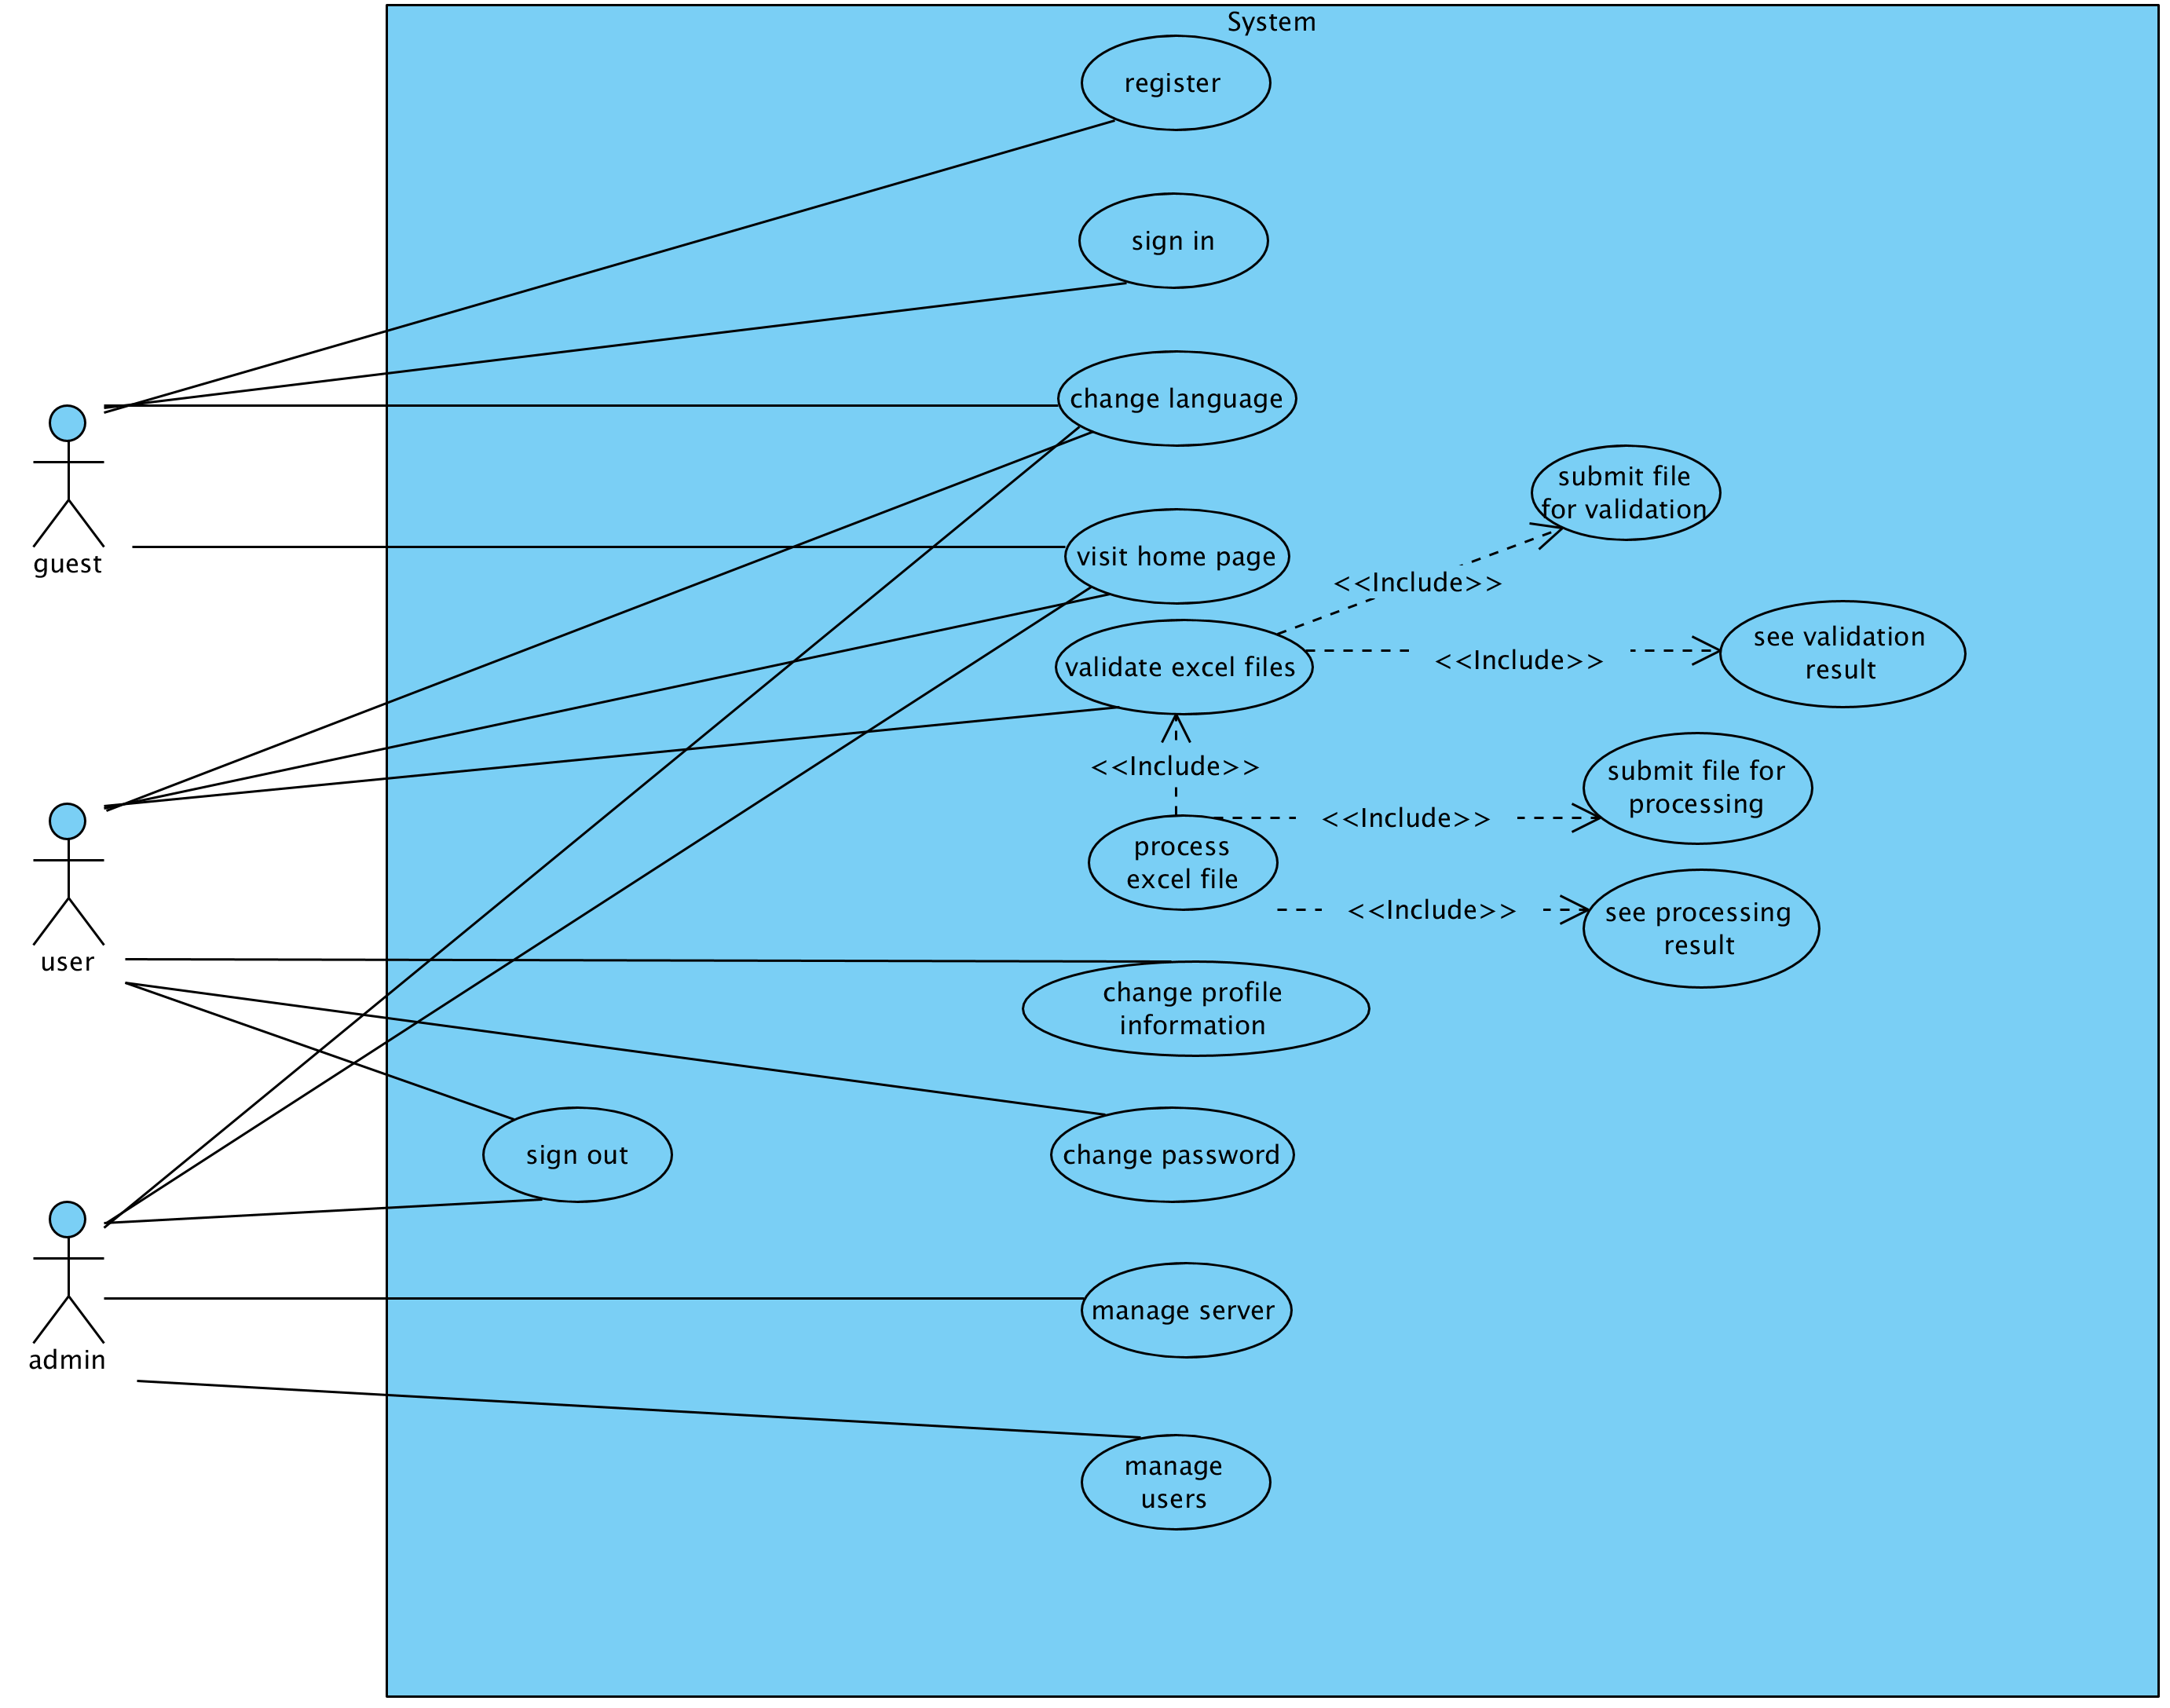
\includegraphics[width=0.8\textwidth]{images/diagrams/use-cases-macro.png}
    \caption{Les cas d'utilisation}
    \label{fig:use-cases-macro}
\end{figure}

\paragraph{}
Le diagramme \ref{fig:use-cases-macro} liste les différents cas d'utilisation et en l'analysant avec attention, on peut observer certains faits qui sont à première vue contre intuitifs.

\paragraph{}
Dans de nombreuses applications, on pourrait considérer une sorte d'héritage entre les différents niveaux de privilèges parmi les utilisateurs. Hors, ce n'est pas le cas ici. En effet, seul le \textbf{visiteur} a accès aux fonctionnalités pour s'enregistrer et se connecter. Plus surprenant, l'\textbf{administrateur} n'a pas accès aux fonctionnalités du coeur de l'application que sont la validation et le traitement des classeurs Excel. Encore plus étonnant, l'administrateur ne peut n'y accéder à son profil, n'y changer son mot de passe.

\begin{figure}[ht]
    \centering
    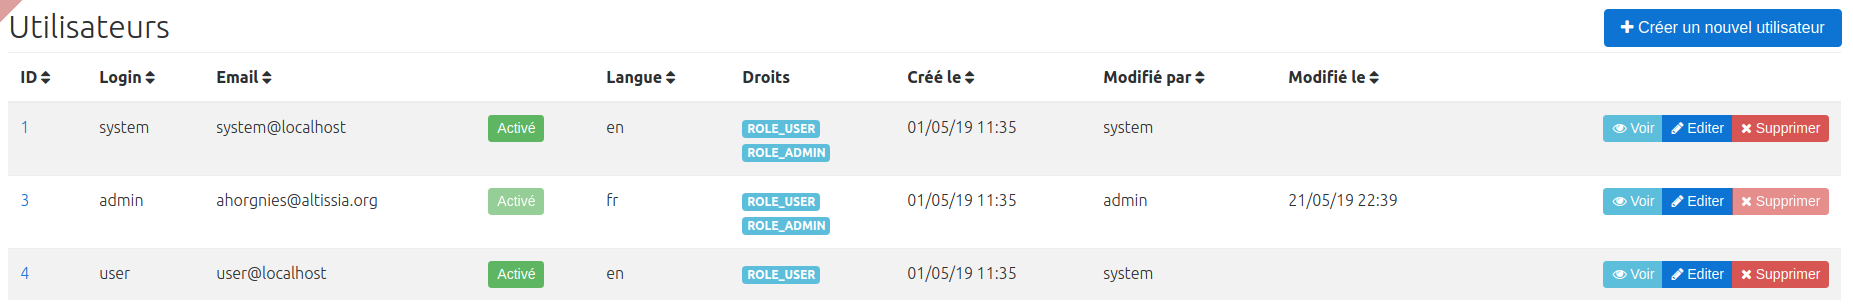
\includegraphics[width=0.8\textwidth]{images/screenshot/screenshot-user-admin-page.png}
    \caption{Une capture d'écran de la page de gestion des utilisateurs}
    \label{fig:user-admin-page}
\end{figure}

\paragraph{}
Cela est du au fait que les permissions sont gérées par un système de licences. Une personne peut cumuler les licences. Ainsi, plutôt que de faire hériter un rôle d'un autre, nous avons choisis de lier les permissions aux licences et de donner autant de licences que nécessaires aux personnes. Cela permet une gestion plus fine des autorisations et aussi plus simple à mettre en place.

Grâce à cela, la nouvelle application peut être déployé avec la base des utilisateurs existante complète sans risquer de compromettre les ressources qu'elle expose. En effet, seuls les personnes qui recevront la licence appropriée auront réellement accès à l'application.

De ce fait, un \textbf{visiteur} n'est pas une personne sans licence mais une personne qui n'a aucune licence adaptée.

Dans les faits, un \textbf{administrateur} aura toujours la licence d'un \textbf{utilisateur}. C'est ce que l'on peut observer sur l'image \ref{fig:user-admin-page}. Il a donc la double casque d'\textbf{administrateur} et d'\textbf{utilisateur}.

\paragraph{}
Le traitement inclue la validation. Bien que ces deux fonctionnalités soient fondamentalement distinctes, nous avons fait le choix d'inclure la validation comme première étape du traitement. Faire ainsi permet d'assurer la validité des données traitées et exclut toute erreur humaine.

\paragraph{}
Une chose qu'il n'est pas possible de voir sur ce diagramme \ref{fig:use-cases-macro} est que la validation et le traitement des classeurs sont des cas d'utilisation abstraits. En effet, il est nécessaire de les spécialiser sans quoi ils ne représentent rien.

Il faut se pencher sur des schémas plus détaillés pour comprendre ce que ces cas d'utilisation couvrent. C'est le sujet de la sous-section \ref{subsec:spreadsheet-use-case}.


\subsection{L'authentification}
\label{subsec:auth-feature}

\paragraph{}
L'authentification mise en place doit être compatible avec le système d'authentification présent sur les services d'Altissia. C'est particulièrement facile car c'est une authentification dite sans serveur. Cela veut dire qu'un client peut prouver son identité sans qu'un serveur tiers confirme les droits auxquels le \gls{g-client} prétend. 

\begin{figure}[h]
    \centering
    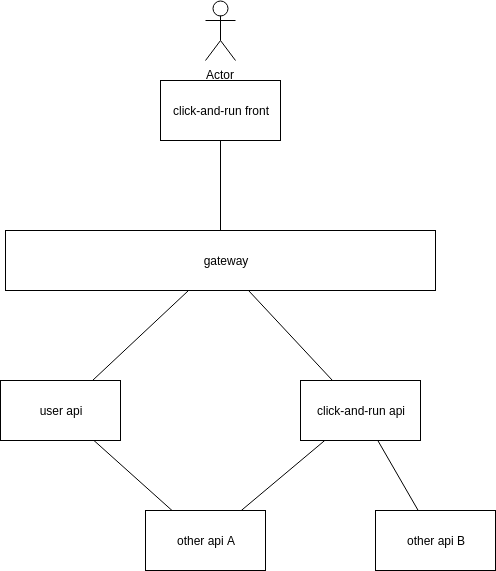
\includegraphics[width=0.7\textwidth]{images/diagrams/gw-archi.png}
    \caption{L'organisation des services et leurs communications (non \gls{a-uml})}
    \label{fig:gw-archi}
\end{figure}

\paragraph{}
Pour comprendre comment c'est possible, il faut d'abord s'intéresser à la manière dont les différents services communiquent entre eux. Comme on peut le voir sur le diagramme \ref{fig:gw-archi}, tous les \glspl{g-server} sont cachés derrière un unique point d'entrée que l'on appelle la passerelle. La passerelle vérifie que les demandes faites aux \glspl{g-server} sont authentifiées. Les demandes faites entre \glspl{g-server} ne sont pas vérifiées car les \glspl{g-server} se font mutuellement confiance.

\begin{figure}[h]
    \centering
    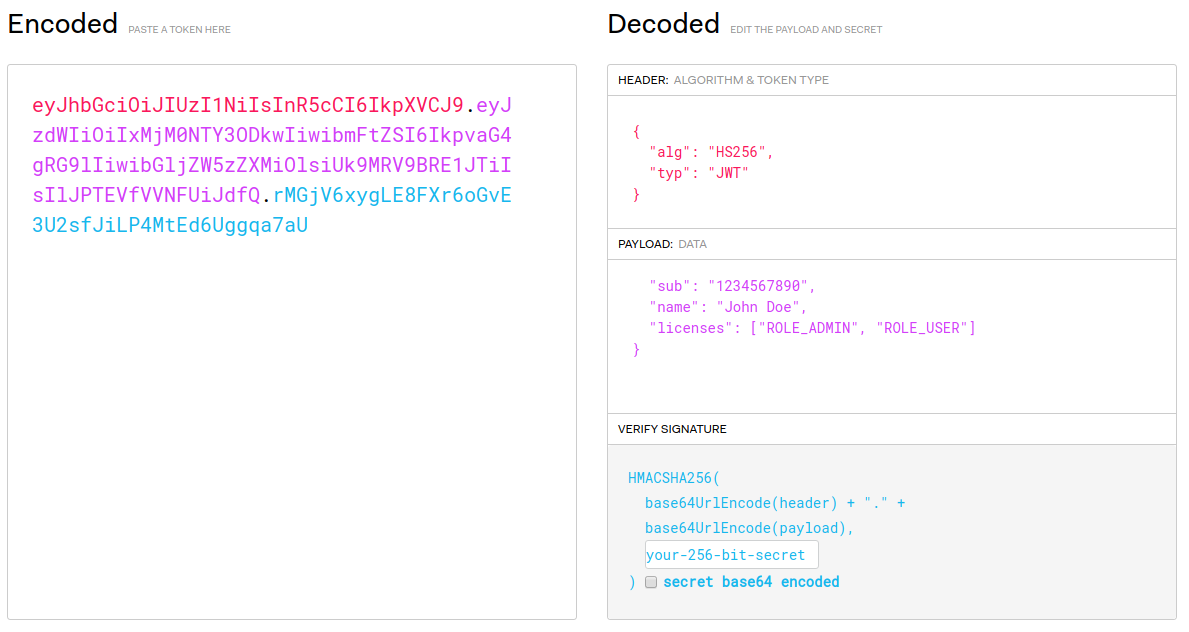
\includegraphics[width=0.7\textwidth]{images/screenshot/jwt-good-secret.png}
    \caption{Un \gls{a-jwt} à gauche et les données décodées à droite}
    \label{fig:jwt-good}
\end{figure}
\begin{figure}[h]
    \centering
    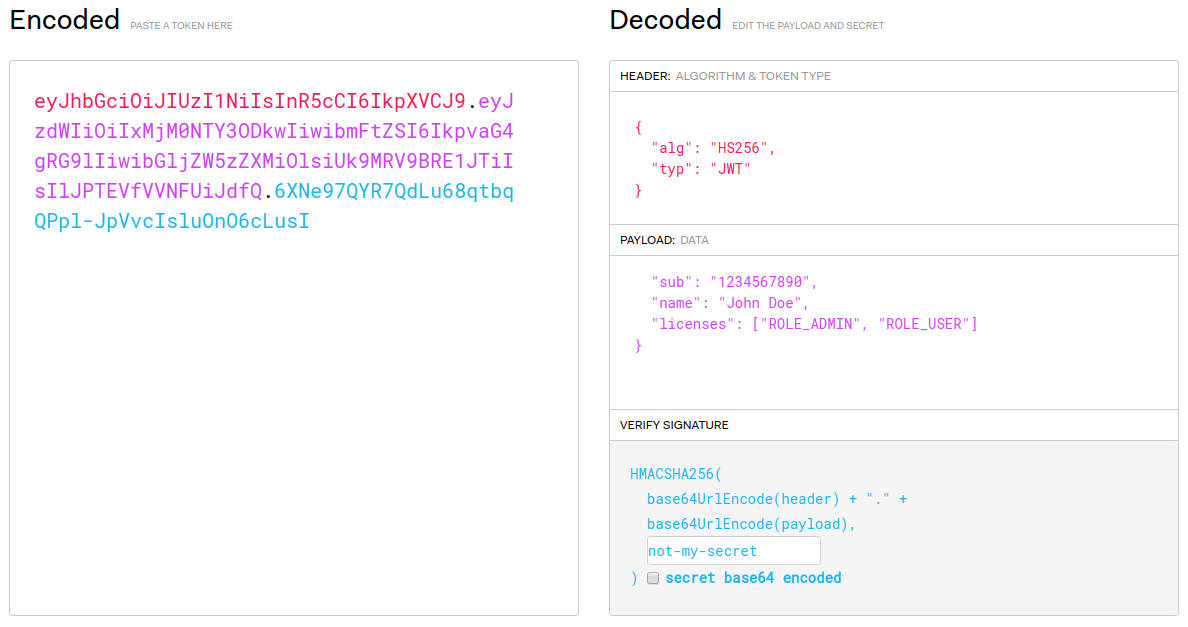
\includegraphics[width=0.7\textwidth]{images/screenshot/jwt-bad-secret.png}
    \caption{Un \gls{a-jwt} avec les mêmes données que sur la figure \ref{fig:jwt-good} mais pas la même signature}
    \label{fig:jwt-bad}
\end{figure}

\paragraph{}
Un \gls{g-client} qui veut s'authentifier fait sa demande à la passerelle.
La passerelle consulte le service des utilisateurs et si l'identifiant et le mot de passe concordent, elle approuve l'authentification.
Elle envoie alors un \gls{a-jwt}, dont on peut observer un exemplaire sur la figure \ref{fig:jwt-good} qui est une sorte de passeport qui déclare l'identité et les droits de l'utilisateur.
Ce \gls{a-jwt} est lisible par tous et est infalsifiable. Son contenu est accompagné d'une signature qui est la résultat de ce même contenu passé par une \gls{g-hash-func}.
La seule manière de reproduire cette signature est disposer de la \gls{g-hash-func} et du secret.
La figure \ref{fig:jwt-bad} illustre ce que l'on obtient sans le bon secret.
Cette formule est présente sur le \gls{a-jwt} et est donc accessible à tous.
Le secret lui n'est connu que par la passerelle et il n'y a donc que elle qui peut produire cette signature.

\paragraph{}
A chaque requête, un client accompagne sa demande de son \gls{a-jwt} et la passerelle reproduit la signature.
Si la signature produite est la même que celle inscrite sur le \gls{a-jwt}, la passerelle transmet la demande, sinon elle la rejette.
Et lorsque les \glspl{g-server} doivent communiquer entre eux pour remplir la demande du client, ils font confiance aux droits indiqués car ils ont été vérifiés par la passerelle.

\paragraph{}
Pour que cela fonctionne, la nouvelle application cliente doit:
\begin{enumerate}
    \item Adresser toutes ses demandes à la passerelle
    \item Implémenter la demande d'authenfication
    \item Fournir le \gls{a-jwt} à chaque requête
\end{enumerate}
Tandis que le nouveau \gls{g-server} doit juste contrôler que les droits d'un utilisateur correspondent au niveau d'autorisation requis pour les ressources qu'il demande.


\subsection{L'internalisation}
\label{subsec:i18n}

\paragraph{}
Chaque valeur textuelle statique\fnmark{} doit être traduite. Seuls des employés d'Altissia auront accès à cette application, il n'est donc pas nécessaire de traduire l'application dans toutes les langues supportées par les autres application d'Altissia\fnmark{}.
\fntext{Toutes données qui ne viennent pas d'une base de données sont dites statiques car elles ne peuvent pas changer pendant la vie de l'application.}
\fntext{Ce qui aurait fait une trentaine de langue dont je n'en connais que trois...}

Il est par contre obligatoire d'être compatible avec le système de localisation qui est déjà mis en place.

Altissia embarque les mécanismes nécessaires à la localisation dans chaque application. Une application peut donc changer de langue sans contacter de \gls{g-server}.

De plus, les informations de localisations sont stockées sur l'application web PhraseApp.
Les localisations devront donc être téléchargées depuis cette dernière.
Le format privilégié pour les applications clientes est le format \gls{a-json}, que l'application devra donc utiliser.

\paragraph{}
L'application cliente devra donc implémenter la localisation seule. C'est le sujet qui est abordé dans la sous section \ref{subsec:i18n-imp}


\subsection{La validation et le traitement des classeurs}
\label{subsec:spreadsheet-use-case}
TODO


\section{Les pages demandées}
\label{subsec:requested-pages}

\paragraph{}
Tous les besoins définis vont se traduire d'une manière ou l'autre en une ou plusieurs pages webs.
Et évidemment, un menu permet de naviguer entre les différentes pages.

\subsection{La page d'accueil}
\label{subsec:home-page}
TODO


\subsection{Les pages du profil}
\label{subsec:profile-page}
TODO


\subsection{Les pages des entités}
\label{subsec:entities-pages}

\paragraph{}
Les pages des entités sont des pages permettant de voir, créer, modifier et supprimer toutes les entrées que peut gérer le site web.
En l'occurrence, les entités sont les apprenants et les licences.

\paragraph{}
Les entités doivent être affichés sont formes de tableaux qui peuvent être triés sur chaque colonne.
Le tri est effectué à partir de la liste complète des entités présentes en base de données et pas uniquement celles qui sont affichées.
Cliquer sur une entité permet d'ouvrir une page qui affiche uniquement les données de celle-ci.

Lorsque l'on clique sur un utilisateur depuis le tableau des licences, on est conduit sur la page de l'utilisateur en question.


\subsection{Les pages de l'administrateur}
\label{subsec:admin-pages}

\paragraph{}
L'\textbf{administrateur} a accès à toute une panoplie d'outils.
Ces pages sont accessibles par un menu qui n'est visible que pour l'\textbf{administrateur}.

Les éléments suivants doivent être présents:
\begin{itemize}
    \item Gateway: Liste les API disponibles
    \item Gestion des utilisateurs: \acrshort{a-crud} sur les listes des \textbf{utilisateurs}
    \item Métriques: Mesures de l'utilisation des ressources de la machine physique sur laquelle est installée l'application
    \item Diagnostics: Liste des services composant l'application et leur état de fonctionnement
    \item Configuration: Liste des propriétés configurables du serveur et leur valeur
    \item Audits: Liste des appels sur les ressources surveillées (ex.: tentative de connexion)
    \item \Glspl{g-log}: Contrôle des niveaux de verbosité des agents de journaux du \gls{g-server}
    \item \gls{a-api}: Liste des ressources exposées par le \gls{g-server} avec exemples d'utilisation
    \item Base de données: Lien vers l'application d'accès à la base de données (ex.: \gls{g-pma})
\end{itemize}

Ces pages doivent correspondre exactement à celles fournies par le générateur de code \Gls{g-jhipster}.
Cet outil est utilisé par Altissia et permet de gagner plusieurs de développements lors de la création de nouveaux projets.
Il génère le code qui constitue le squelette d'un site web et le développeur se l'approprie pour ajouter de nouvelles fonctionnalités par dessus.


\subsection{La page de validation et traitement des classeurs}
\label{subsec:spreadsheet-page}

\paragraph{}
La page de validation et traitement des données est la page centrale de l'application et c'est elle qui va justifier le plus de travail.
Son fonctionnement doit être le plus simple possible.
Un \textbf{utilisateur} doit pouvoir s'en servir sans formation et ses actions ne peuvent pas tromper ses intentions.

\paragraph{}
La page est divisée en trois éléments:
\begin{itemize}
    \item Le récepteur de fichier: il permet de choisir le fichier que l'on valide
    \item Le tableau des résultats: il affiche les résultats de la validation
    \item Le bouton de traitement: il lance le traitement du fichier validé
\end{itemize}

\paragraph{}
Le récepteur de fichier permet de choisir un fichier de deux manières, soit en cliquant dessus, soit en glissant et en déposant un fichier sur lui.
Dans le premier cas, il ouvre le menu système\fnmark{} de l'utilisateur. Dans le second cas, l'utilisateur a cliqué sur le fichier et a maintenu le clic, a glissé le fichier au-dessus du composant et a relâché le clic.
\fntext{Le menu système est le menu prévu par le système d'exploitation installé sur la machine de l'utilisateur}

Dans le cas où le fichier n'est pas compatible, car il n'est pas un fichier Excel ou est corrompu, un message d'erreur renseigne l'utilisateur.
Dans le cas où le fichier est compatible, la validation de son contenu est immédiatement lancée sans autre action de l'utilisateur.

Le nom du fichier sélectionné avec succès est affiché sur le récepteur.

Un doubleclic sur le récepteur vide le fichier.

Des instructions indiquent les actions à prendre en fonction de l'état du fichier: présent ou non présent. % TODO gérer valide et non valide ?

\paragraph{}
Le tableau des résultats affiche les erreurs de validation relevées par le \gls{g-server}.
Le résultat de chaque feuille est affiché dans son propre onglet.
Les erreurs sont divisées en trois tableaux distincts: les problèmes de titre, les erreurs de contenu et les avertissements sur le contenu.
Pour les problèmes de titres, le numéro de colonne, le titre de la colonne, la valeur dans le fichier pour cette colonne et le message d'erreur sont affichés.
Le message d'erreur est exprimé dans un langage intelligible par un \textbf{utilisateur}.
Les mêmes champs sont utilisés par les erreurs et avertissements si ce n'est que la colonne devient une ligne.
Les erreurs sont affichées dans l'ordre des lignes.

\paragraph{}
Le bouton de traitement n'est utilisable que si le fichier a passé la validation.
Son activation envoie le fichier déjà sélectionné et déjà validé pour son traitement.
En cas de succès, ce qui est sensé toujours être le cas, un message de succès apparait et le fichier est vidé du récepteur de fichier.




\section{Le socle d'application de validation et de traitement des classeurs}
\label{sec:spreadsheet-framework}

\paragraph{}
Les outils mis en place doivent au minimum permettre de résoudre les cas d'utilisation proposés.
Mais ils doivent aussi être le plus générique possible afin de pouvoir être appliqués à le plus de cas possibles.
Le socle d'application doit être conçu de manière à ce qu'il soit le plus facile possible d'intégrer de nouveaux outils.

\paragraph{}
Le but de créer un socle d'application plutôt qu'une application concrète est d'être capable de gérer des nouveaux cas avec un temps de développement minimale.
Il est créé libre de droits afin que n'importe qui puisse s'en servir et y contribuer.
Il est donc logique qu'il contienne des outils prêts à l'utilisation, qu'il soit prêt à accueillir des outils inconnus et qu'il soit compatible avec des standards informatiques répandus.

\subsection{Le fonctionnement de Click-and-Run}
\label{subsec:operation}


\subsection{Les outils prêts à l'emploi}
\label{subsec:ready-tools}

\paragraph{}
La plupart des règles de validation ne sont pas propres à un seul classeur, il faut donc les concevoir de façon à ce qu'elles soient utilisables dans d'autres classeurs.

\paragraph{}
Je ne vais donc pas implémenter une règle pour vérifier un format de chaine de caractère précis, mais une règle pour vérifier les formats de manière général.

Je n'ai pas créé une règle qui vérifie qu'un nombre est compris entre 0 et 365, mais deux règles: une pour vérifier qu'une valeur est plus grande qu'une borne et une qui vérifie que la même valeur est inférieure à une autre borne.

Vérifier qu'une valeur fait parti de la liste des services revient à vérifier qu'une valeur est un élément d'un ensemble.

Vérifier que le nom est long de deux à cinquante caractères résulte en une règle qui vérifie la taille d'une chaine de caractères.

Vérifier que l'email est bien défini revient à vérifier qu'il n'est pas \gls{g-null}.


\subsection{Des outils à intégrer}
\label{subsec:host-tools}

\paragraph{}
Certaines règles sont trop spécifiques et il n'est pas possible de les généraliser.
Il est par contre possible de simplifier la vie du développeur qui va devoir les ajouter en prévoyant un système qui va détecter la règle et l'appliquer au bon moment et dans les bons cas.

\paragraph{}
La personne qui veut rajouter une règle dispose de trois points d'entrée:
\begin{itemize}
    \item Le modèle d'une feuille: elle peut associer sa règle au modèle qui représente une ligne
    \item La validation de feuille: elle peut ajouter un service qui sera appelé lors de la validation de la feuille
    \item la validation de classeur: elle peut ajouter un service qui sera appelé lors de la validation du classeur
\end{itemize}
Afin que cela fonctionne, elle doit respecter les formats prévus par mon application.

\paragraph{}
La règle d'un modèle est appliquée sous la forme d'une annotation \textit{javax.validation.constraints}.
C'est un format standard pour la validation que je discute dans la section suivante.

\paragraph{}
Pour la validation d'une feuille ou d'un classeur, le développeur doit créer un service qui doit:
\begin{enumerate}
    \item Indiquer qu'il est capable de traiter le type de données que la validation est en train de vérifier
    \item Implémenter une méthode avec une signature précise qui effectue la vérification
\end{enumerate}
Ce mécanisme correspond au patron de conception de la stratégie.
Il est discuté dans la section \ref{subsec:class-diagram}.


\subsection{Les outils compatibles}
\label{subsec:compatible-tools}


